\section[rnn]{Recurrent Networks / Sequential data processing}

\begin{frame}
  \frametitle{Recurrent Neural Network}
    \begin{center}
      \def\layersep{3.5cm}
    \begin{tikzpicture}[shorten >=1pt,->,draw=black!50, node distance=\layersep]
        \tikzstyle{every pin edge}=[<-,shorten <=1pt]
        \tikzstyle{neuron}=[circle,draw=black,fill=white,minimum size=17pt,inner sep=0pt]
    
        \draw node[neuron, fill=white] (I-x) at (0,-1.25) {}; 
        \draw node[neuron, fill=white] (I-y) at (0,-2.75) {}; 
        
        \draw node[neuron, fill=white] (H-1) at (\layersep,-0.5) {$f$}; 
        \draw node[neuron, fill=white] (H-2) at (\layersep,-2.0) {$f$}; 
        \draw node[neuron, fill=white] (H-3) at (\layersep,-3.5) {$f$}; 
    
        \draw node[neuron,fill=white,pin={[pin edge={->}]right:$y$}, right of=H-2] (O) {$g$}; 
        
        \draw[line width=1pt, color=black] (I-x) -> (H-1);
        \draw[line width=1pt, color=black] (I-x) -> (H-2);
        \draw[line width=1pt, color=black] (I-x) -> (H-3);
        \draw[line width=1pt, color=black] (I-y) -> (H-1);
        \draw[line width=1pt, color=black] (I-y) -> (H-2);
        \draw[line width=1pt, color=black] (I-y) -> (H-3);
        
        \draw<2>[->,-latex',line width=1pt,color=black] (H-1.north west) arc[x radius=0.25cm, y radius =.25cm, start angle=220, end angle=-60];
        \draw<2>[->,-latex',line width=1pt,color=black] (H-2.north west) arc[x radius=0.25cm, y radius =.25cm, start angle=220, end angle=-60];
        \draw<2>[->,-latex',line width=1pt,color=black] (H-3.north west) arc[x radius=0.25cm, y radius =.25cm, start angle=220, end angle=-60];
                
        \draw[line width=1pt, color=black] (H-1) -> (O);
        \draw[line width=1pt, color=black] (H-2) -> (O);
        \draw[line width=1pt, color=black] (H-3) -> (O);
    
        \draw node[above of=H-1, node distance=1.5cm] (hl) {Hidden layer};
        \draw node[left of=hl] {Input layer};
        \draw node[right of=hl] {Output layer};
        
    \end{tikzpicture} 
    
    \end{center}    
    \onslide<2>{
    \textbf{Recurrent networks contain loops;\\ last output of the neuron is used as additional input}
    }

\end{frame}

\begin{frame}[fragile]
  \frametitle{Backpropgation through Time}
    \begin{center}
          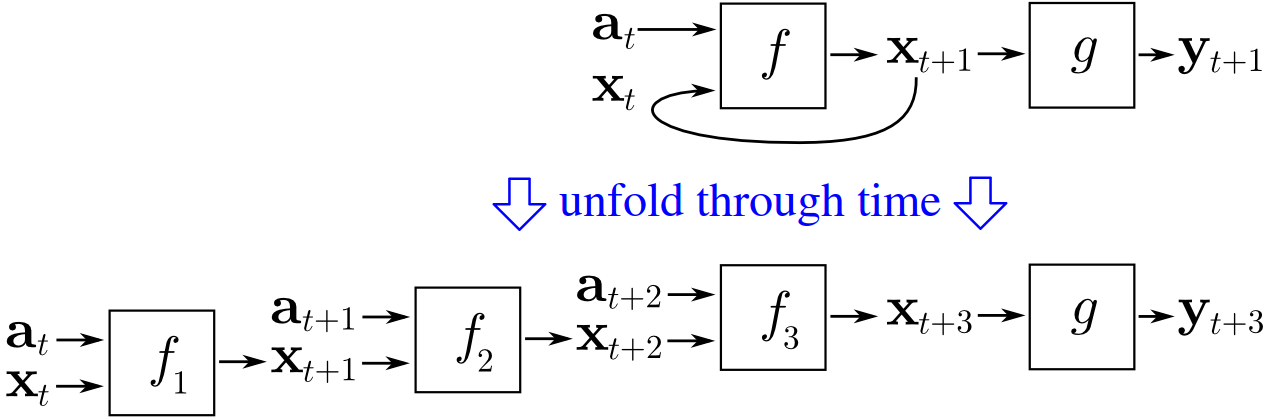
\includegraphics[width=\textwidth]{Unfold_through_time.png}
          
          
          {\tiny \url{https://en.wikipedia.org/wiki/Backpropagation_through_time#/media/File:Unfold_through_time.png} }
          
    \vspace{1.5em}
    \textbf{Problem: Activation function will be applied iteratively\\ $\Rightarrow$ value (and gradient) vanishes or explodes}
    \end{center}
\end{frame}

\begin{frame}
  \frametitle{Solution: Long Short-Term Memory}
    \begin{center}
        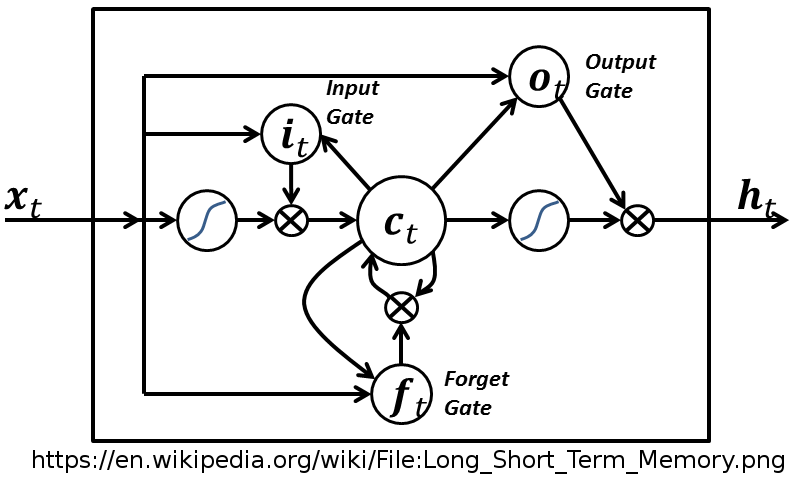
\includegraphics[width=0.6\textwidth]{Long_Short_Term_Memory.png}
        \begin{itemize}
          \item Can remember a value for a long time period
          \item Input gate decides when to update the stored value
          \item Output gate decides when to output the stored value
          \item Forget gate decides when to forget the stored value
        \end{itemize}
        \textbf{$\rightarrow$ Can process sequential data (e.g. text and speech)}
    \end{center}
\end{frame}

\begin{frame}
  \frametitle{Example: A simple character level language model}
    \begin{center}
        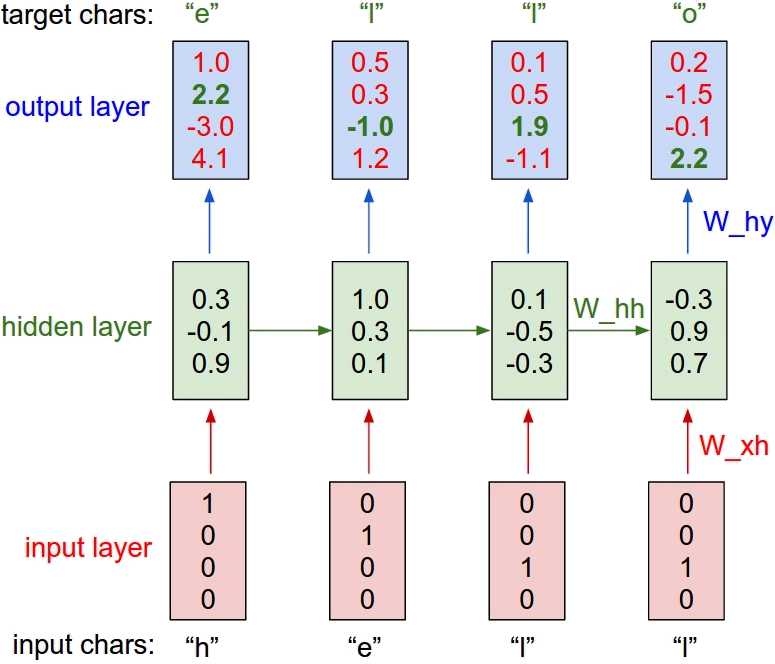
\includegraphics[width=0.6\textwidth]{charseq.png}

        \url{http://karpathy.github.io/2015/05/21/rnn-effectiveness/}
    \end{center}
\end{frame}

\begin{frame}
  \frametitle{Example: Applied on C-Code}
    \begin{center}
        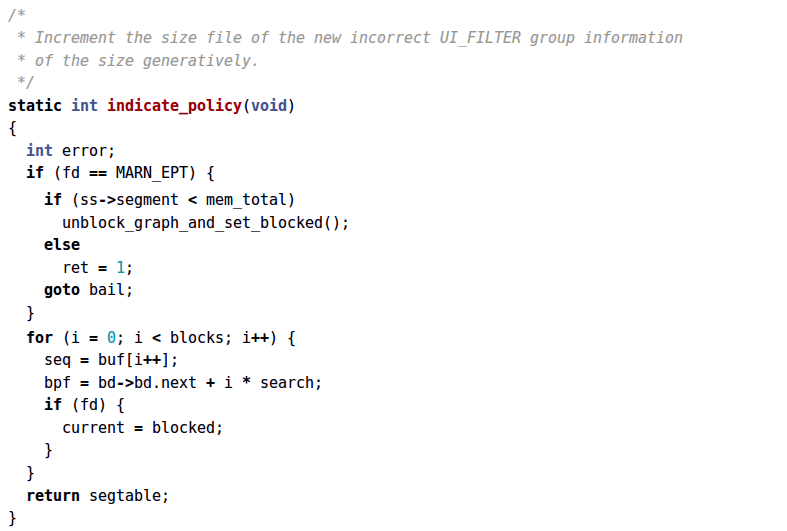
\includegraphics[width=0.8\textwidth]{linuxcode.png}
        
        \url{http://karpathy.github.io/2015/05/21/rnn-effectiveness/}
    \end{center}
\end{frame}

\begin{frame}
  \frametitle{Example: Learned Concepts from C-Code}
    \begin{center}
    
    Activation profile of selected neurons
    \vspace{2em}
    		     
    \begin{columns}
    \begin{column}{0.5\textwidth}
	    \textbf{If-Statements}\\
        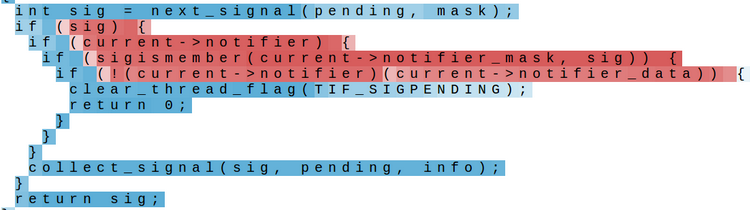
\includegraphics[width=0.9\textwidth]{rnn_if.png}
        
        \vspace{2em}
        \textbf{Depth of Scopes}\\
        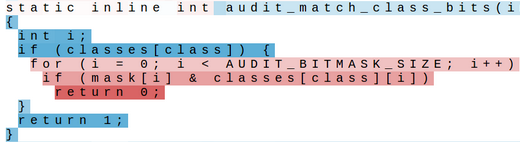
\includegraphics[width=0.9\textwidth]{rnn_depth.png}
    \end{column}
        \begin{column}{0.5\textwidth}
    	    \textbf{Line length}\\
		    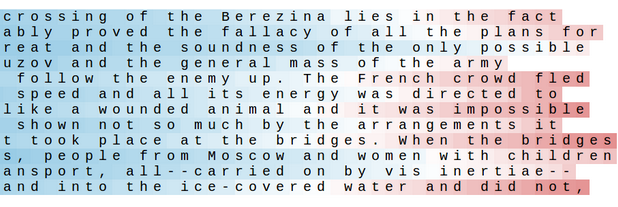
\includegraphics[width=0.9\textwidth]{rnn_length.png}
		    
		     \vspace{2em}
		    \textbf{Comments}\\
	        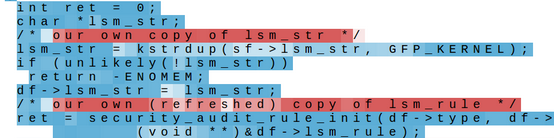
\includegraphics[width=0.9\textwidth]{rnn_comments.png}
        \end{column}
    \end{columns}

		     \vspace{2em}
        \url{http://karpathy.github.io/2015/05/21/rnn-effectiveness/}
    \end{center}
\end{frame}


\begin{frame}
  \frametitle{Example: Write descriptions of images}
    \begin{center}
      \begin{tikzpicture}
        \node[anchor=south west,inner sep=0] at (0,0) {
\includegraphics[width=\textwidth]{neuralimagecaption.png}};
        \node[anchor=south west,inner sep=0] at (1,-4) {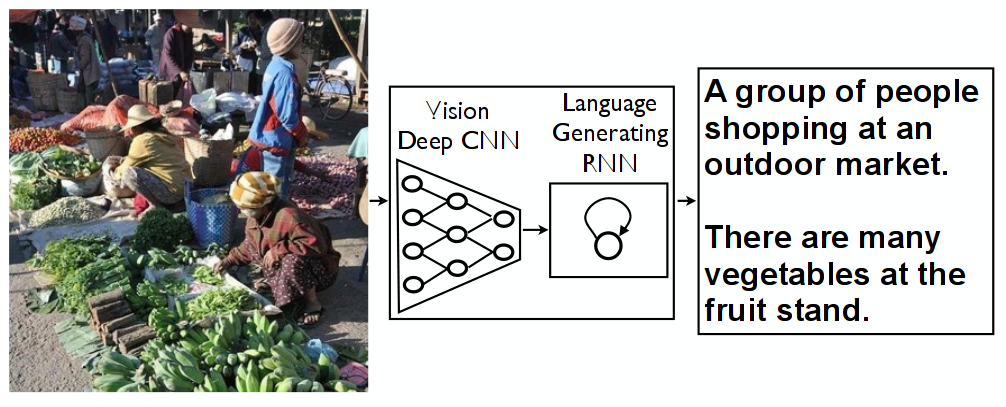
\includegraphics[width=0.8\textwidth]{imagecaptionexample.png}};
      \end{tikzpicture}


      \vspace{-1em}
      \begin{itemize}
        \item Extract information using a convolutional neural network
        \item Generate description using a recurrent neural network
      \end{itemize}
    \end{center}
\end{frame}
